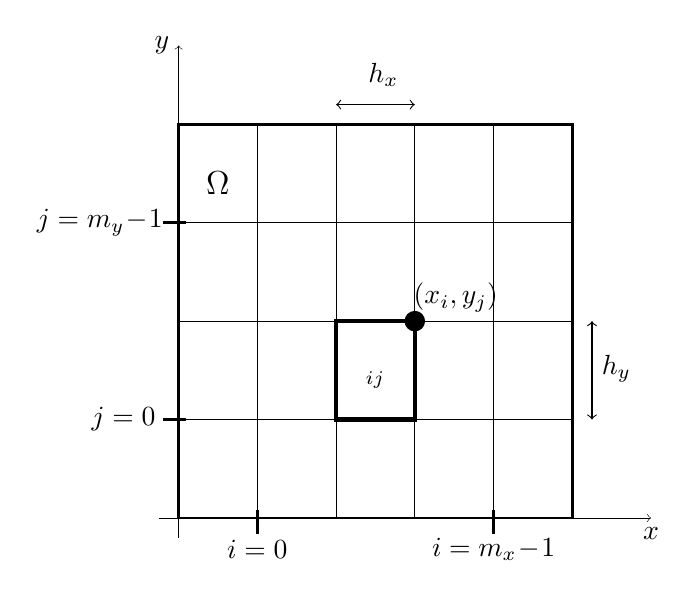
\begin{tikzpicture}[scale=5.0]
  % axes
  \draw[->,very thin] (-0.05,0.0) -- (1.2,0.0) node[below] {$x$};
  \draw[->,very thin] (0.0,-0.05) -- (0.0,1.2) node[left] {$y$};
  % grid
  \draw[line width=1.0pt] (0.0,0.0) -- (0.0,1.0) -- (1.0,1.0) -- (1.0,0.0) -- cycle;
  \pgfmathsetmacro\fifth{1.0/5.0}
  \pgfmathsetmacro\fourth{1.0/4.0}
  \draw[xstep=\fifth,ystep=\fourth,black,thin] (0.0,0.0) grid (1.0,1.0);
  \node at (0.1,0.85) {\large $\Omega$};
  % outline an element, showing location and dimensions
  \draw[line width=1.5pt] (0.6,0.5) -- (0.4,0.5) -- (0.4,0.25) -- (0.6,0.25) -- cycle;
  \node at (0.5,0.35) {$\square_{ij}$};
  \filldraw (0.6,0.5) circle (0.7pt) node[xshift=5.2mm,yshift=3mm] {$(x_i,y_j)$};
  \draw[<->] (0.4,1.05) -- (0.6,1.05) node[above,yshift=1mm,xshift=-4mm] {$h_x$};
  \draw[<->] (1.05,0.25) -- (1.05,0.5) node[right,yshift=-6mm] {$h_y$};
  % tick marks for i
  \draw[line width=1.0pt] (0.2,-0.04) -- (0.2,0.02);
  \draw[line width=1.0pt] (0.8,-0.04) -- (0.8,0.02);
  \node[yshift=-4mm] at (0.2,0.0) {$i=0$};
  \node[yshift=-4mm] at (0.8,0.0) {$i=m_x\!-\!1$};
  % tick marks for j
  \draw[line width=1.0pt] (-0.04,0.25) -- (0.02,0.25);
  \draw[line width=1.0pt] (-0.04,0.75) -- (0.02,0.75);
  \node[xshift=-7mm] at (0.0,0.25) {$j=0$};
  \node[xshift=-10mm] at (0.0,0.75) {$j=m_y\!-\!1$};
\end{tikzpicture}

